\documentclass[8pt]{beamer}
\usepackage{tikz}
\usepackage[utf8]{vietnam}
\usepackage{amsmath}
\usepackage{graphicx}
\usepackage{wrapfig}
\usepackage{mathrsfs}
\usepackage{hyperref}
\usetheme{Copenhagen}
\usecolortheme{beaver}
\setbeamertemplate{navigation symbols}{}
\setbeamertemplate{headline}{}
\title[Chương 3: Biến đổi Fourier] %optional
{Chương 3: Biến đổi Fourier}
\subtitle{Tín hiệu và hệ thống}
\author[Tín hiệu và hệ thống] % (optional)
{Tín Vũ}
\date[VLC 2021] % (optional)
{tinvu1309@gmail.com}
\begin{document}
\frame{\titlepage}
\begin{frame}{Mục lục}
\tableofcontents
\end{frame}
\begin{frame}{Giới thiệu playlist}
\section{Giới thiệu playlist}
	\begin{itemize}
		\item Mình là Tín Vũ, hiện tại đang là sinh viên học tại Trường Đại học Công nghệ, Đại học Quốc gia Hà Nội. Mình tạo playlist video này để hỗ trợ các bạn học môn Tín hiệu và hệ thống trong các trường đại học kĩ thuật theo hướng \alert{trực quan hóa} nhất có thể.
		\item Do đó, mục tiêu của mình khi thực hiện playlist này không chỉ giúp các bạn ôn thi được điểm cao mà còn \alert{hiểu sâu công thức để làm nền tảng cho các môn học sau}.
		\item Để đạt được hai mục tiêu trên, các bạn nên xem \textbf{toàn bộ} video của mình, còn nếu chỉ cần ôn thi cấp tốc và đạt điểm cao thì hãy \textbf{bỏ qua} các video "optional".
		\item Nội dung playlist này chủ yếu bám sát nội dung môn học Tín hiệu và hệ thống tại trường của mình; nếu các bạn học trường khác, hãy tham khảo kĩ đề cương hay đề thi của trường bạn để đối chiếu sao cho ôn tập đúng trọng tâm và hợp lý. 
		\item Môn học này bao gồm \textbf{6} chương, các chương đều liên quan rất chặt chẽ và logic với nhau nên hãy học cẩn thận ngay từ \alert{chương 0} để ôn thi cuối kì đỡ vất vả.
	\end{itemize}
\end{frame}
\begin{frame}{Tài liệu tham khảo}
\section{Tài liệu tham khảo}
\begin{itemize}
		\item Tài liệu tham khảo chính: Signals and Systems (2nd edition) Alan V. Oppenheim and Alan S. Willsky.
		\item Tài liệu tham khảo phụ: Bài tập của mình học khóa trước, đề thi các năm cũ,...
		\item Tài liệu tham khảo phụ: Nếu bạn là sinh viên trường mình và muốn học "tủ" nhiều bài thì nên đọc Signals and Systems (2nd edition) Simon Haykin vì các thầy cô chủ yếu dạy và ra đề trong cuốn này, thế nhưng mình đánh giá cuốn này không đầy đủ và chi tiết như sách của Alan V. Oppenheim. 
	\end{itemize}
\end{frame}
\begin{frame}{Giới thiệu về Fourier}
\section{Giới thiệu về Fourier}
\begin{wrapfigure}{l}{0.4\textwidth} %this figure will be at the right
    \centering
    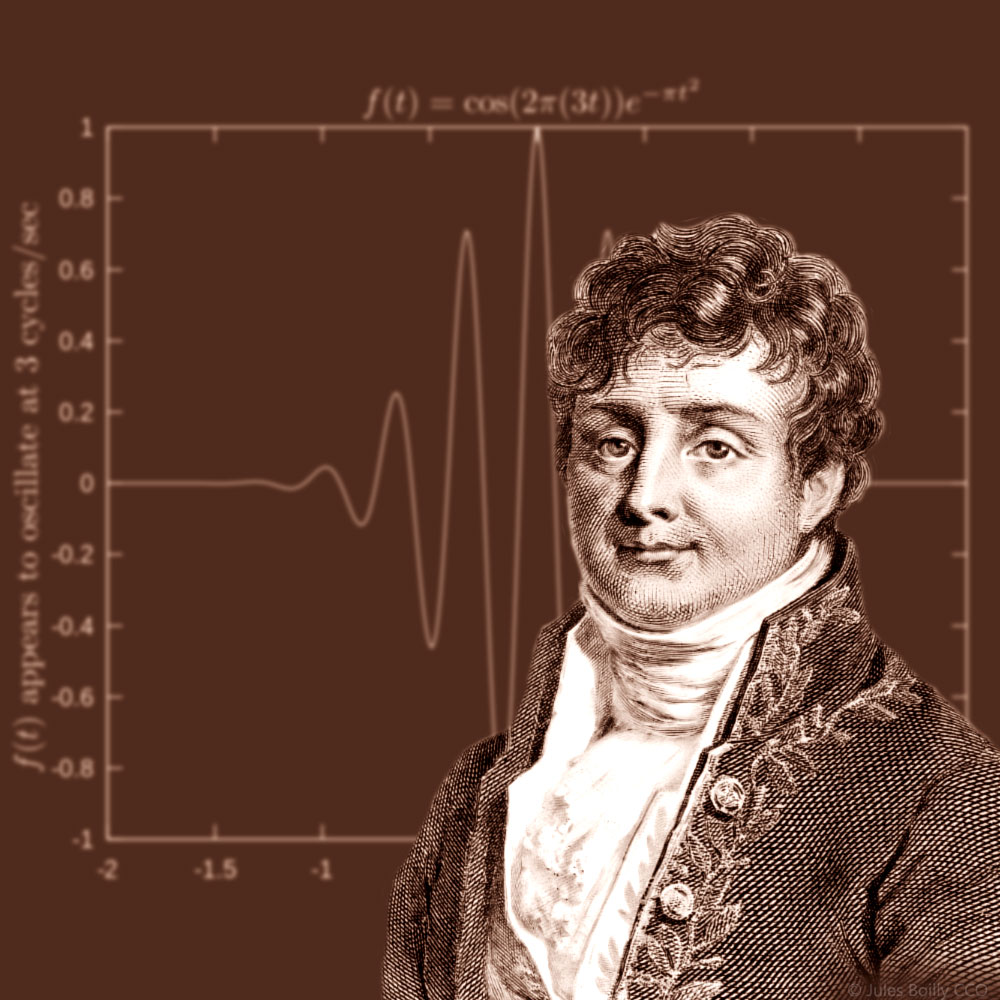
\includegraphics[width=0.4\textwidth]{Fourier-1000.jpg}
\end{wrapfigure}
Joseph Fourier là nhà toán học huyền thoại \\
người Pháp sống ở thế kỉ 18. Công trình nổi tiếng nhất của 
ông là phép biến đổi Fourier được ông nghiên cứu khi giải quyết bài toán \\
truyền nhiệt đã đặt nền móng cho toàn bộ lĩnh vực xử lý tín hiệu phát triển mạnh mẽ sau này. 
\\ Phép biến đổi Fourier chính là trái tim\\ của toàn bộ ngành khoa học kĩ thuật hiện đại.

\end{frame}
\begin{frame}{Giới thiệu về Fourier}
\begin{figure}[h]
			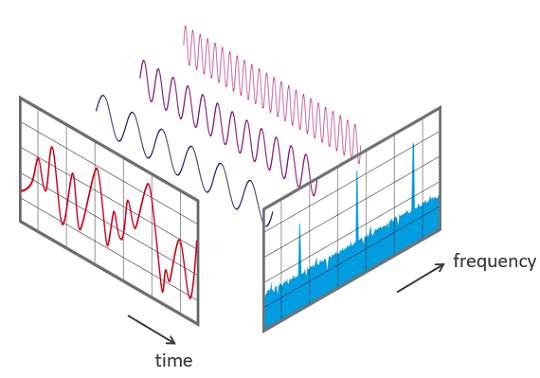
\includegraphics[width=0.9\textwidth]{FFT-Time-Frequency-View-540.png}
			\caption{Fourier Transform Visualization}\label{fig:re11}
		\end{figure}

\end{frame}
\begin{frame}{Chuỗi Fourier (FS)}
	\section{Chuỗi Fourier (FS)}
\subsection{Chuỗi Fourier liên tục (CTFS)}
\begin{itemize}
	\item Chuỗi Fourier liên tục (CTFS)
\end{itemize}
\subsubsection{Khái niệm chuỗi Fourier liên tục}
\begin{itemize}
	\item[-] Khái niệm chuỗi Fourier liên tục
\end{itemize}
Một tín hiệu $x(t)$ \alert{liên tục} và \textbf{tuần hoàn} bất kì đều có thể được biểu diễn dưới dạng tổng của các tín hiệu tuần hoàn khác:
$$x(t)=\sum_{k=-\infty}^{+\infty}a_{k}e^{jk\omega_{0} t}=\sum_{k=-\infty}^{+\infty}a_{k}e^{jk\frac{2\pi}{T_{0}}t}$$
Hệ số $a_{k}$ được tìm ra như sau, với $n$ là số nguyên tùy ý:
\begin{equation*}
\begin{split}
	x(t)e^{-jn\omega_{0}t}&=\sum_{k=-\infty}^{+\infty}a_{k}e^{jk\omega_{0}t}e^{-jn\omega_{0}t}
	\\ \Leftrightarrow \int_{T_{0}}x(t)e^{-jn\omega_{0}t}dt&=\int_{T_{0}}\sum_{k=-\infty}^{+\infty}a_{k}e^{jk\omega_{0}t}e^{-jn\omega_{0}t}dt\\
							       &=\sum_{k=-\infty}^{+\infty}a_{k}\left[\int_{T_{0}}e^{j(k-n)\omega_{0}t}dt\right]
\end{split}
\end{equation*}
Với $n\neq k$, hiển nhiên tích phân bằng $0$ (do bản chất tích phân của hàm tuần hoàn trên một chu kì), vậy khi và chỉ khi $n=k$ thì tích phân mới có giá trị xác định bằng $T_{0}$.
\end{frame}
\begin{frame}{Chuỗi Fourier (FS)}

\\ Vậy ta thu được công thức tính hệ số chuỗi FS liên tục (CTFS):
$$\alert{a_{k}=\frac{1}{T_{0}}\int_{T_{0}}x(t)e^{-jk\omega_{0}t}dt}$$
Khi giải bài tập, với tín hiệu đơn giản ta khai triển trực tiếp bằng cách tách tín hiệu gốc thành dạng mũ phức, còn với tín hiệu phức tạp ta sử dụng công thức trên để tìm hệ số FS.
\\ Ví dụ 1: khai triển tín hiệu sau thành chuỗi Fourier liên tục:
$$x(t)=\cos(\omega_{0}t)$$
Ta rất dễ dàng khai triển tín hiệu trên theo công thức Euler từ định nghĩa:
$$x(t)=\frac{1}{2}\left(e^{j\omega_{0}t}+e^{-j\omega_{0}t}\right)=\frac{1}{2}e^{j\omega_{0}t}+\frac{1}{2}e^{-j\omega_{0}t}$$
Ta tìm được các hệ số chuỗi Fourier như sau:
\begin{equation*}
	a_{k}=
	\begin{cases}
		\frac{1}{2}\; (k=-1\; , k=1)	\\
		0 \;(\text{otherwise})\\
\end{cases}
\end{equation*}
Vậy ta kết luận: tín hiệu $x(t)$ được cấu tạo từ hai tín hiệu tuần hoàn nhỏ hơn, với cả hai tín hiệu thành phần đều có \alert{biên độ} bằng $\frac{1}{2}$, \alert{tần số góc} bằng $\omega_{0}$ , $-\omega_{0}$ và \alert{pha ban đầu} đều bằng $0$ rad. \\$\Rightarrow$ \textbf{Tại sao lại xuất hiện thành phần tần số góc âm ?}
\end{frame}
\begin{frame}{Chuỗi Fourier (FS)}
\begin{figure}[h]
			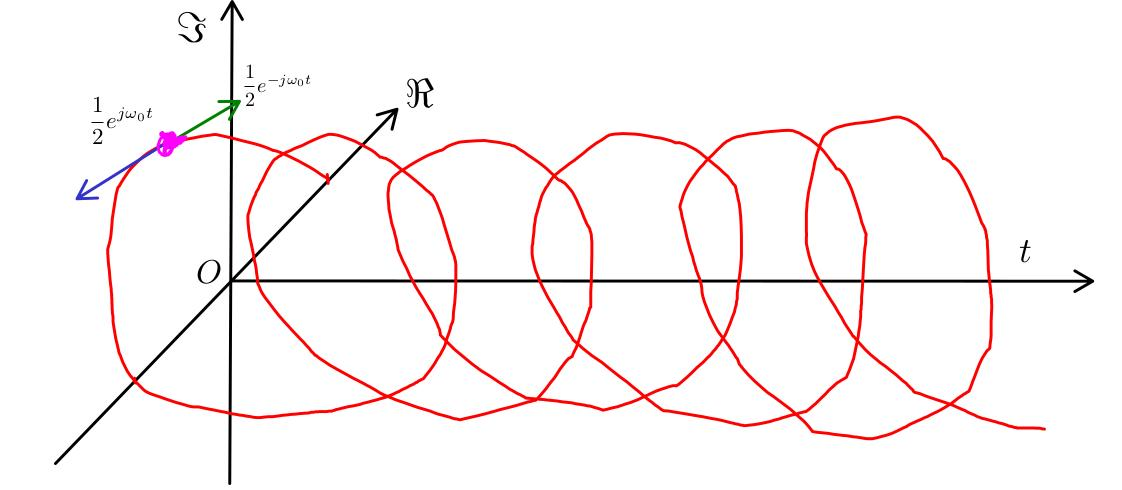
\includegraphics[width=0.5\textwidth]{helix.jpg}
			\caption{Harmonic component helix curve}\label{fig:re11}
		\end{figure}
\begin{figure}[h]
			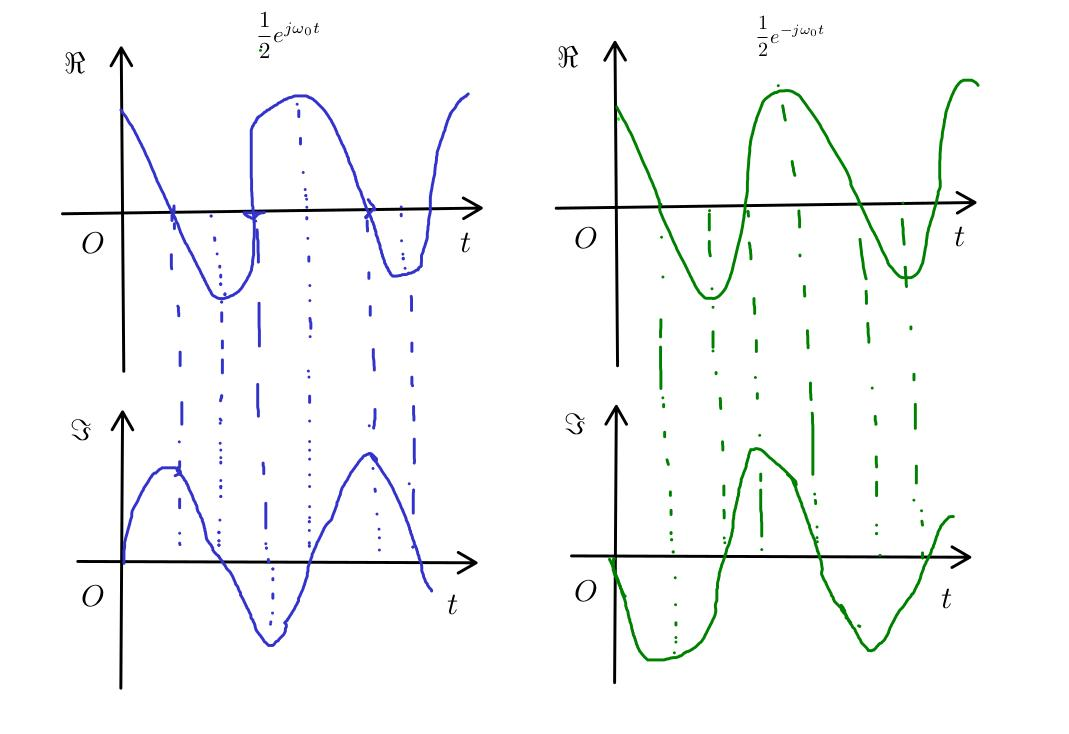
\includegraphics[width=0.5\textwidth]{imaginary.jpg}
			\caption{Negative Frequency Explanation}\label{fig:re11}

		\end{figure}
\end{frame}
\begin{frame}{Chuỗi Fourier (FS)}
\begin{figure}[h]
			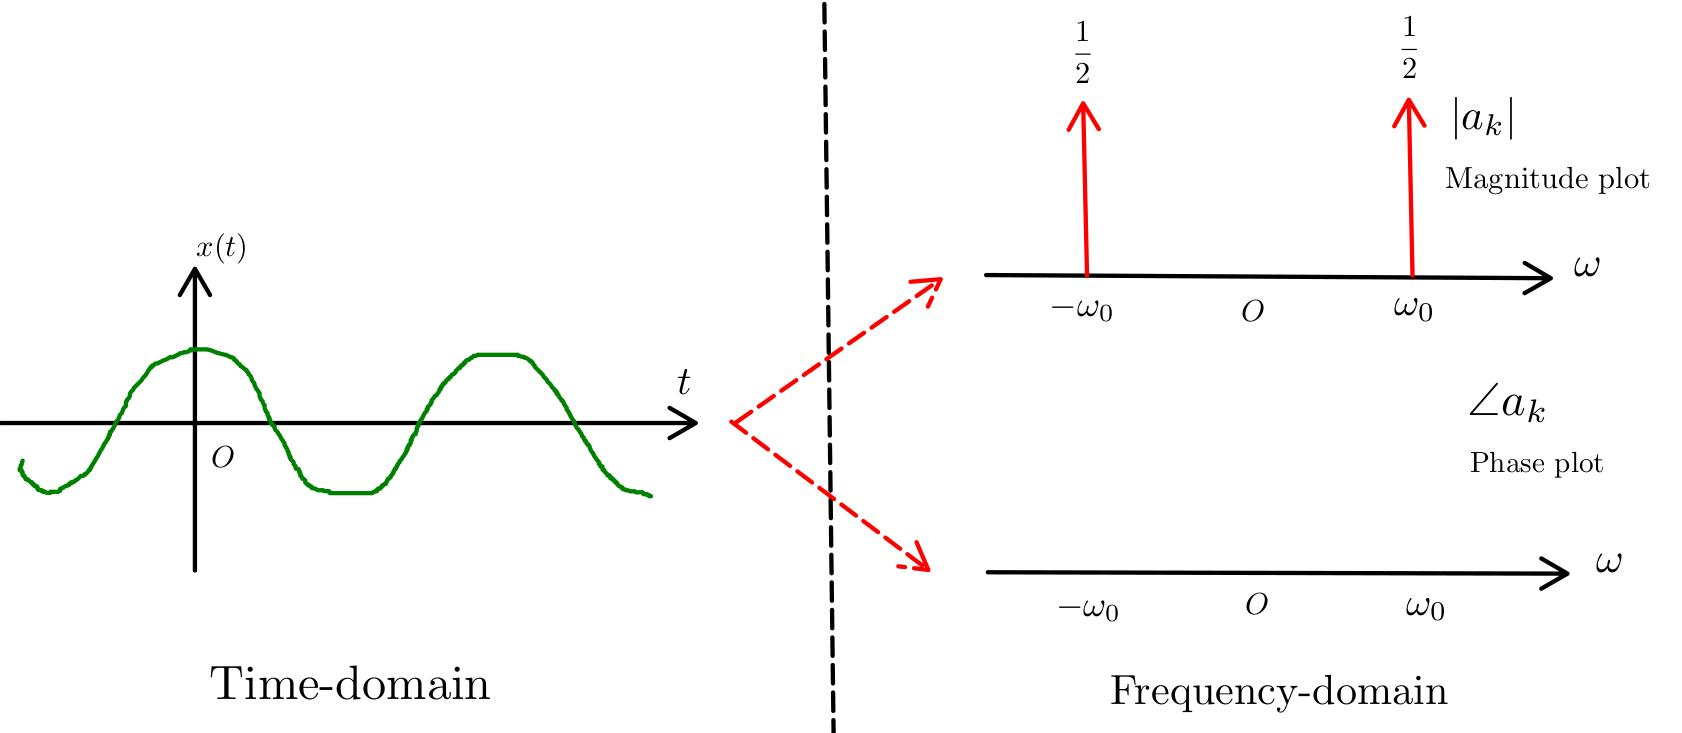
\includegraphics[width=0.47\textwidth]{fre.jpg}
			\caption{Simple cosine signal spectrum}\label{fig:re11}

		\end{figure}

		Suy ngẫm: vẽ phổ tín hiệu sine, giải thích nguyên nhân xuất hiện thành phần \textbf{tần số âm}. Nếu loại bỏ thành phần \textbf{tần số âm} thì sao? 
$$x(t)=\sin{(\omega_{0}t)}$$
\begin{figure}[h]
			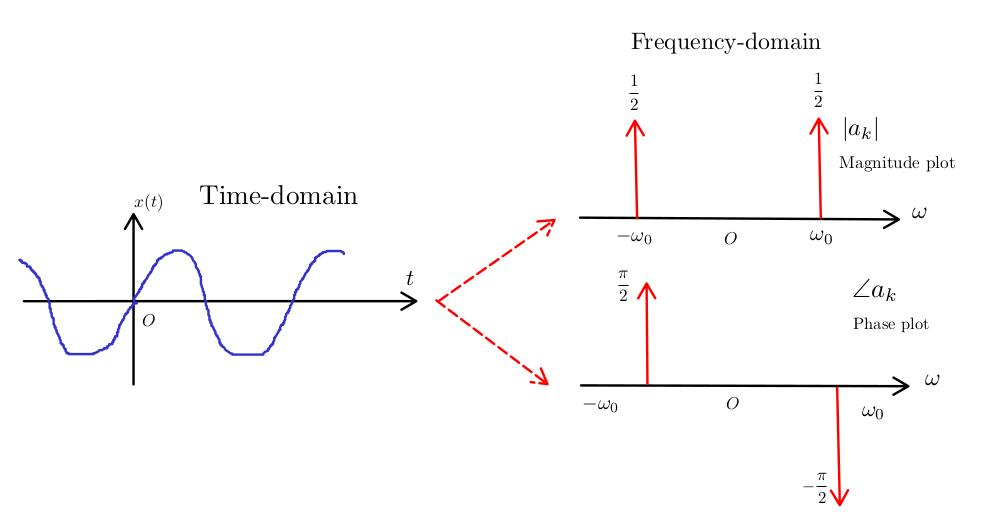
\includegraphics[width=0.47\textwidth]{sine.jpg}
			\caption{Simple sine signal spectrum}\label{fig:re11}

		\end{figure}


\end{frame}
\begin{frame}{Chuỗi Fourier (FS)}

\begin{figure}[h]
			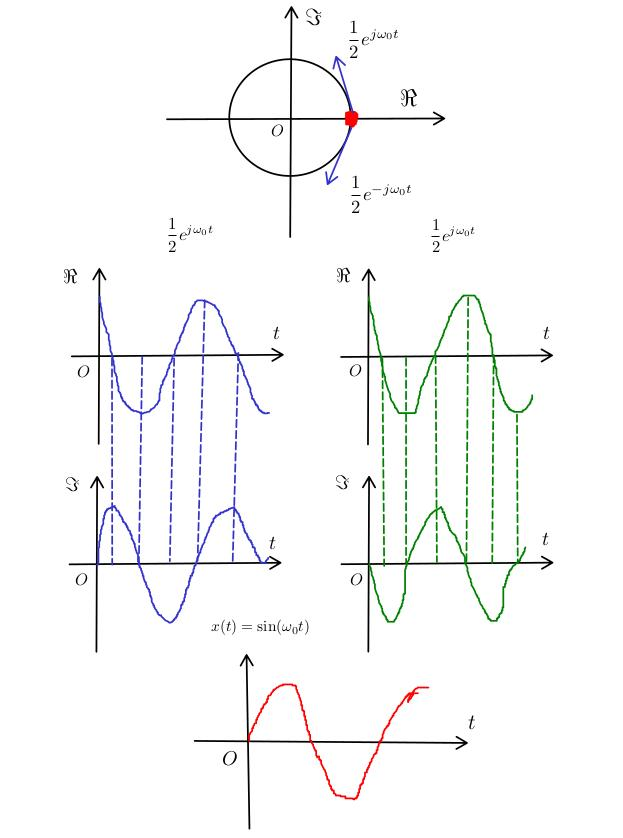
\includegraphics[width=0.5\textwidth]{sin.jpg}
			\caption{Components of sine signal explanation}\label{fig:re11}

		\end{figure}
\end{frame}
\begin{frame}{Chuỗi Fourier (FS)}
Ví dụ 2: khai triển tín hiệu sau thành chuỗi Fourier liên tục:
\begin{figure}[h]
			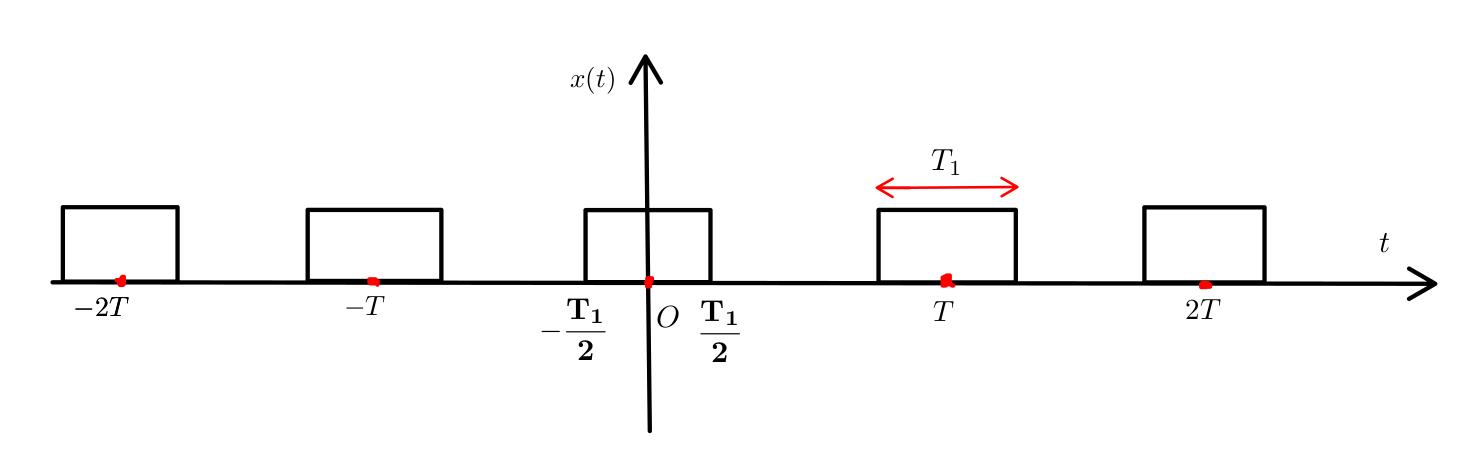
\includegraphics[width=0.6\textwidth]{square.jpg}
			\caption{Square wave signal in time-domain}\label{fig:re11}

		\end{figure}
		Để khai triển tín hiệu trên thành chuỗi Fourier liên tục, ta phải dùng công thức tính $a_{k}$ chứ không thể tách trực tiếp được nữa:
\begin{equation*}
\begin{split}
a_{k}=\frac{1}{T}\int_{T}x(t)e^{-jk\omega_{0}t}dt
\end{split}
\end{equation*}
Xét trường hợp đặc biệt $k=0$, ta có: $$a_{0}=\frac{1}{T}\int_{T}dt=\frac{1}{T}\int_{-\frac{T_{1}}{2}}^{\frac{T_{1}}{2}}dt=\frac{T_{1}}{T}$$
Với $k\neq 0$, ta có:
\begin{equation*}
	\begin{split}
		a_{k}=\frac{1}{T}\int_{T}x(t)e^{-jk\omega_{0}t}dt=\frac{1}{T}\int_{-\frac{T_{1}}{2}}^{\frac{T_{1}}{2}}e^{-jk\omega_{0}t}dt=\frac{\sin{\left(k\omega_{0}\frac{T_{1}}{2}\right)}}{k\pi}
\end{split}
\end{equation*}
\end{frame}
\begin{frame}{Chuỗi Fourier (FS)}
Vậy ta thu được hệ số chuỗi Fourier liên tục:
\begin{equation*}
	a_{k}=
	\begin{cases}
		\frac{T_{1}}{T} \; (k=0)\\
		\frac{\sin{\left(k\omega_{0}\frac{T_{1}}{2}\right)}}{k\pi} \;(k\neq0)\\

	\end{cases}
\end{equation*}
\begin{figure}[h]
			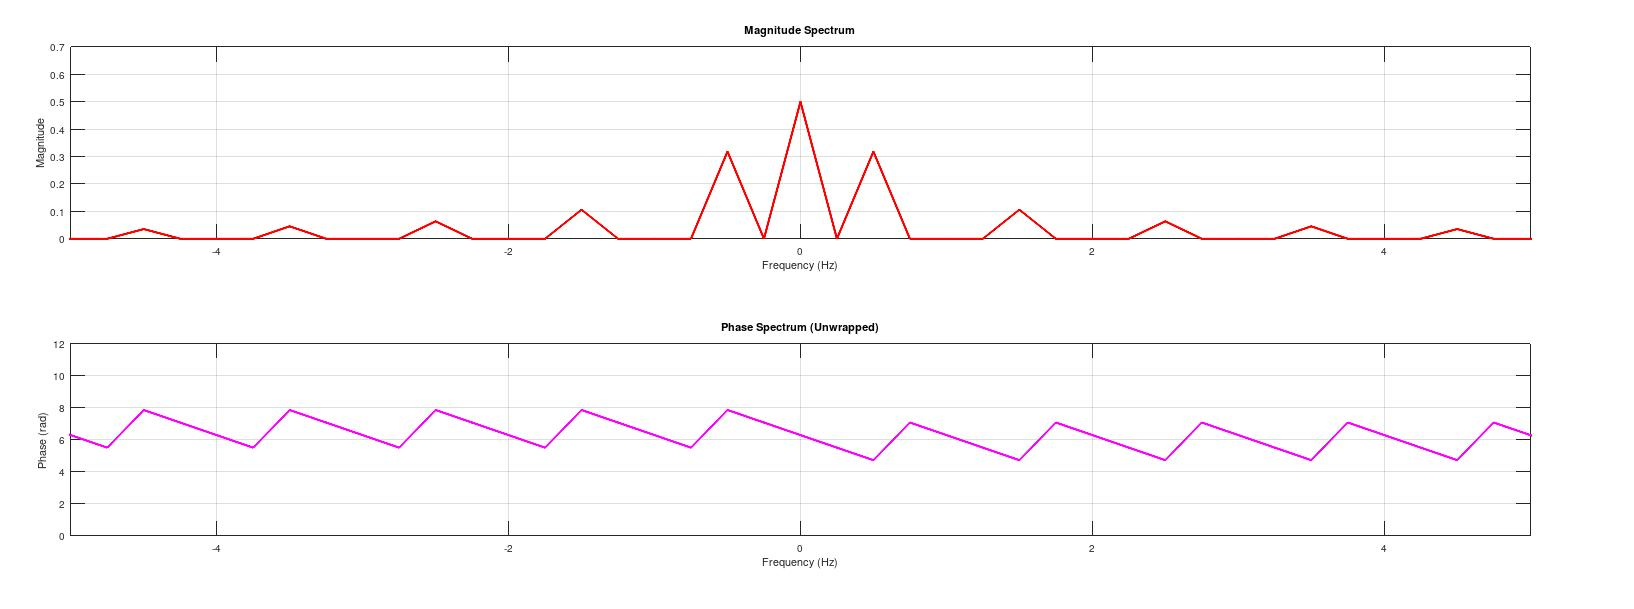
\includegraphics[width=0.9\textwidth]{s.jpg}
			\caption{Square wave signal in frequency-domain}\label{fig:re11}

		\end{figure}
	Suy ngẫm: các bạn hãy thử tự giải lại ví dụ 1 bằng công thức tính $a_{k}$ như ở trên.
\end{frame}
\begin{frame}{Chuỗi Fourier (FS)}
\subsubsection{Tính chất chuỗi Fourier liên tục}
\begin{itemize}
	\item[-] Tính chất chuỗi Fourier liên tục
\end{itemize}
\begin{block}{Continuous-time Fourier  Series Pair}
\begin{equation*}
\begin{split}
	x(t)&=\sum_{k=-\infty}^{+\infty}a_{k}e^{jk\omega_{0}t}\\
	a_{k}&=\frac{1}{T_{0}}\int_{T_{0}}x(t)e^{-jk\omega_{0}t}dt\\
\end{split}
\end{equation*}
\end{block}
Ta định nghĩa phép toán biến đổi tín hiệu liên tục $x(t)$ về chuỗi Fourier liên tục như sau:

$$\mathscr{FS}(x(t))=a_{k}$$
Xét cặp tín hiệu $x(t)$ và $y(t)$ tương ứng có phép toán biến đổi chuỗi Fourier liên tục tương ứng:
$$\mathscr{FS}(x(t))=a_{k}$$
$$\mathscr{FS}(y(t))=b_{k}$$
Ta xét các tính chất cơ bản của chuỗi Fourier liên tục như sau:
\end{frame}
\begin{frame}{Chuỗi Fourier (FS)}
\begin{enumerate}
	\item[1] Tính tuyến tính:
\begin{equation*}
\begin{split}
	\mathscr{FS}(\alpha x(t)+\beta y(t))&=\frac{1}{T_{0}}\int_{T_{0}}(\alpha x(t)+\beta y(t))e^{-jk\omega_{0}t}dt\\
					    &= \alpha\frac{1}{T_{0}}\int_{T_{0}}x(t)e^{-jk\omega_{0}t}dt+\beta\frac{1}{T_{0}}\int_{T_{0}}y(t)e^{-jk\omega_{0}t}dt\\
					    &= \alpha\mathscr{FS}(x(t))+\beta\mathscr{FS}(y(t))
\end{split}
\end{equation*}
Như đã thảo luận ở \alert{chương 1}, ta có thể tổng quát hóa bài toán xét tính tuyến tính cho tổ hợp tuyến tính của vô số tín hiệu.
\item[2] Dịch thời gian:
\begin{equation*}
\begin{split}
	\mathscr{FS}(x(t-t_{0}))&=\frac{1}{T_{0}}\int_{T_{0}}x(t-t_{0})e^{-jk\omega_{0}t}dt\\
				&= \frac{1}{T_{0}}\int_{T_{0}}x(t-t_{0})e^{-jk\omega_{0}(t-t_{0})}e^{-jk\omega_{0}{t_{0}}}d(t-t_{0})\\
				&= e^{-jk\omega_{0}t_{0}}a_{k}
\end{split}
\end{equation*}
\end{enumerate}
\end{frame}
\begin{frame}{Chuỗi Fourier (FS)}
\begin{enumerate}
	\item[3] Lật tín hiệu:
\begin{equation*}
\begin{split}
	\mathscr{FS}(x(-t))&=\frac{1}{T_{0}}\int_{T_{0}}x(-t)e^{-jk\omega_{0}t}dt=\frac{-1}{T_{0}}\int_{T_{0}}x(-t)e^{-jk\omega_{0}t}d(-t)\\
			   &= \frac{1}{T_{0}}\int_{T_{0}}x(t)e^{jk\omega_{0}t}dt=a_{-k}
\end{split}
\end{equation*}
\item[4] Co dãn trong miền thời gian:
$$\mathscr{FS}(x(\alpha t))=a_{k}$$
do co dãn trong miền thời gian chỉ làm ảnh hưởng đến tần số $\omega_{0}\to \alpha\omega_{0}$ chứ không làm ảnh hưởng đến hệ số $a_{k}$.
\item[5] Phép đạo hàm:
\begin{equation*}
\begin{split}
\mathscr{FS}\left(\frac{dx(t)}{dt}\right)&=jk\omega_{0}a_{k}
\end{split}
\end{equation*}
\item [6] Phép tích phân:
	$$\mathscr{FS}\left(\int_{-\infty}^{t}x(\tau)d\tau\right)=\frac{a_{k}}{jk\omega_{0}}$$
\end{enumerate}
\end{frame}
\begin{frame}{Chuỗi Fourier (FS)}
	\begin{enumerate}
\item[7] Phép tích thường (tích điều chế):
\begin{equation*}
\begin{split}
	\mathscr{FS}(x(t)y(t))&=\frac{1}{T_{0}}\int_{T_{0}}(x(t)y(t))e^{-jk\omega_{0}t}dt\\&=\frac{1}{T_{0}}\int_{T_{0}}x(t)\left(\sum_{k=-\infty}^{+\infty}b_{k}e^{jn\omega_{0}t}\right)e^{-jk\omega_{0}t}dt\\&=\frac{1}{T_{0}}\sum_{k=-\infty}^{+\infty}b_{k}\int_{T_{0}}x(t)e^{j(n-k)\omega_{0}t}dt\\&=\sum_{k=-\infty}^{+\infty}b_{k}a_{n-k}=b_{k}*a_{k}
\end{split}
\end{equation*}
\item[8] Đẳng thức năng lượng Parseval: 
$$\frac{1}{T_{0}}\int_{T_{0}}|x(t)|^2dt=\sum_{k=-\infty}^{+\infty}|a_{k}|^2$$
Công suất trung bình của tín hiệu trong một chu kì (vế trái) bằng \textbf{tổng các hệ số chuỗi Fourier của tín hiệu} (vế phải). Đẳng thức này rất khó để có thể chứng minh đơn giản, nên ở đây ta chỉ có thể hiểu đại khái ý tưởng của nó như sau: xét một thành phần điều hòa có tần số góc bằng $k\omega_{0}$ ngẫu nhiên trong tín hiệu $x(t)$, hiến nhiên ta có công suất trung bình của nó trong một chu kì là:
	\end{enumerate}
\end{frame}
\begin{frame}{Chuỗi Fourier (FS)}
	\begin{enumerate}
		\item[]
	$$\frac{1}{T_{0}}\int_{T_{0}}|x_{k}(t)|^2dt=\frac{1}{T_{0}}\int_{T_{0}}|a_{k} e^{jk\omega_{0}t}|^2dt=|a_{k}|^2$$
	Vậy với một tín hiệu $x(t)$ gồm nhiều thành phần điều hòa, ta có:

$$\frac{1}{T_{0}}\int_{T_{0}}|x(t)|^2dt=\sum_{k=-\infty}^{+\infty}|a_{k}|^2$$
\end{enumerate}
Từ 8 tính chất cơ bản của chuỗi Fourier liên tục này, ta có thể giải bài tập nhanh hơn rất nhiều so với áp dụng trực tiếp cặp công thức CTFS pair đã đề cập ở trên. Tất nhiên, do đây không phải là phần nằm trọng tâm trong nội dung thi, nên chúng ta sẽ chỉ lướt rất nhanh qua một ví dụ đơn giản: 
sóng vuông $x(t)$ được biểu diễn như hình vẽ dưới đây có hệ số Fourier liên tục $a_{k}$, hãy xác định hệ số Fourier $b_{k}$ của tín hiệu $y(t)$.
\begin{figure}[h]
			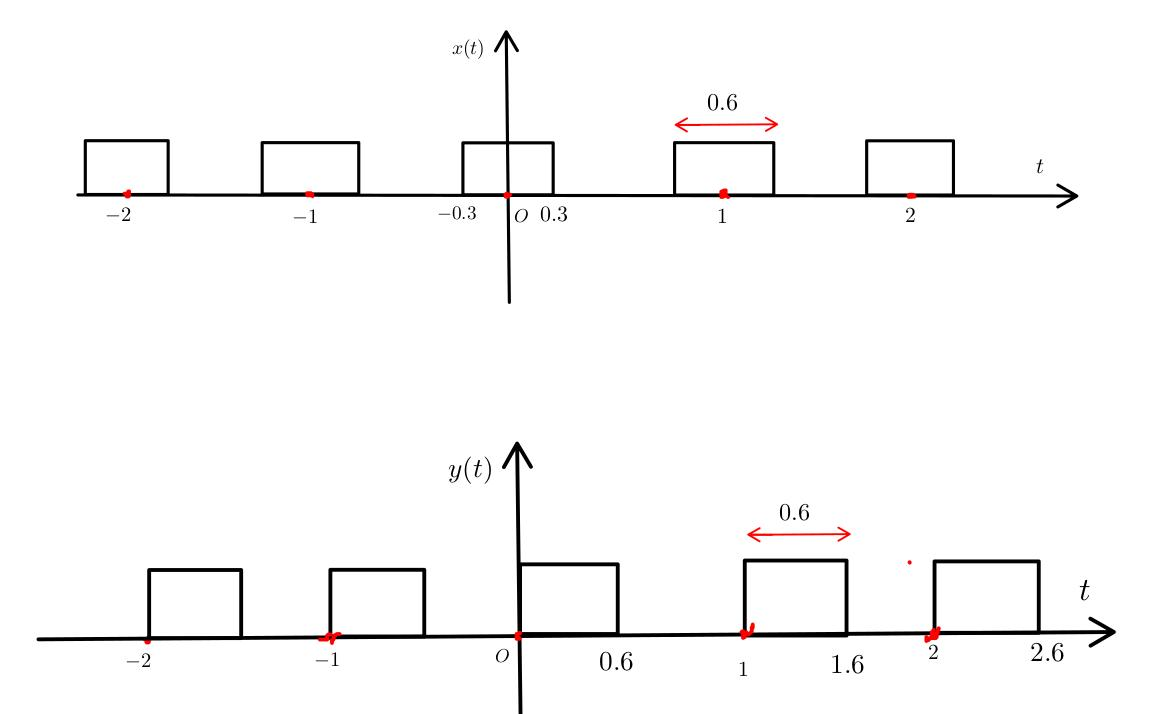
\includegraphics[width=0.46\textwidth]{pro.jpg}
			\caption{Square wave signal in time-domain}\label{fig:re11}

		\end{figure}

\end{frame}
\begin{frame}{Chuỗi Fourier (FS)}
Ta dễ thấy:
$$y(t)=x(t-0.3)\Rightarrow \mathscr{FS}(y(t))=\mathscr{FS}(x(t-0.3))=a_{k}e^{-jk\frac{2\pi}{T_{0}}0.3}=a_{k}e^{-jk0.6\pi}$$
Suy ngẫm: từ ví dụ 2 ở mục trước, các bạn hãy tính ra kết quả cuối cùng của bài toán này với gợi ý trên
\subsubsection{Đáp ứng của hệ thống LTI với tín hiệu tuần hoàn}
\begin{itemize}
	\item[-] Đáp ứng của hệ thống LTI với tín hiệu tuần hoàn
\end{itemize}
Trong \alert{Chương 2}, chúng ta đã xét một họ bài toán tìm đầu ra của hệ thống LTI với đầu vào cho trước bằng phép tích chập; ở đây ta xét một kết quả cực kì đặc biệt đặc trưng cho đầu ra của hệ thống với đầu vào là tín hiệu \textbf{tuần hoàn}. 
\begin{figure}[h]
			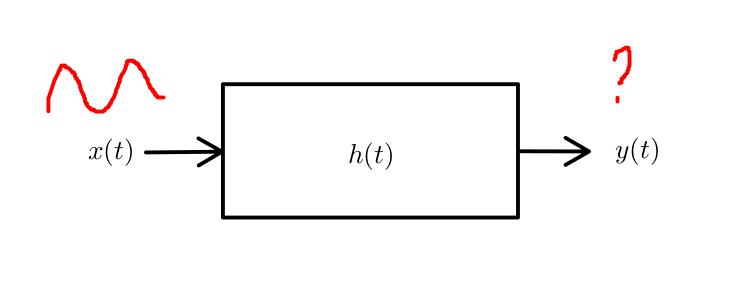
\includegraphics[width=0.46\textwidth]{ht.jpg}
			\caption{If the input of LTI system is periodic signal, what's the output ?}\label{fig:re11}

		\end{figure}
Vì $x(t)$ là tín hiệu \textbf{tuần hoàn}, nên ta có thể tách $x(t)$ thành chuỗi Fourier liên tục:
$$x(t)=\sum_{k=-\infty}^{+\infty}a_{k}e^{jk\omega_{0} t}$$
\end{frame}
\begin{frame}{Chuỗi Fourier (FS)}
Do tích chập có tính \alert{tuyến tính} nên ta có:
$$y(t)=x(t)*h(t)=\sum_{k=-\infty}^{+\infty}[(a_{k}e^{jk\omega_{0}t})*h(t)]=\sum_{k=-\infty}^{+\infty}x_{k}(t)*h(t)$$
Với $x_{k}(t)=a_{k}e^{jk\omega_{0}t}$ là một thành phần điều hòa của tín hiệu $x(t)$ lớn. Ta xét tích chập:
\begin{equation*}
\begin{split}
	y_{k}(t)=x_{k}(t)*h(t)&=\int_{-\infty}^{+\infty}x_{k}(\tau)h(t-\tau)d\tau=\int_{-\infty}^{+\infty}x_{k}(t-\tau)h(\tau)d\tau\\&=\int_{-\infty}^{+\infty}a_{k}e^{jk\omega_{0}(t-\tau)}h(\tau)d\tau=\int_{-\infty}^{+\infty}a_{k}e^{jk\omega_{0} t}h(\tau)e^{-jk\omega_{0}\tau}d\tau\\&=x_{k}(t)\int_{-\infty}^{+\infty}h(\tau)e^{-jk\omega_{0}\tau}d\tau
\end{split}
\end{equation*}
Ta kí hiệu:
$$H(jk\omega_{0})=\int_{-\infty}^{+\infty}h(\tau)e^{-jk\omega_{0}\tau}d\tau$$
là hàm số theo biến tần số $\omega_{0}$, và gọi hàm số này là \alert{đáp ứng tần số của hệ thống},
ta tiếp tục suy ra:
$$y(t)=\sum_{k=-\infty}^{+\infty}y_{k}(t)=\sum_{k=-\infty}^{+\infty}x_{k}(t)H(jk\omega_{0})$$
\end{frame}
\begin{frame}{Chuỗi Fourier (FS)}
	Ví dụ: tìm đáp ứng lối ra của hệ thống có đáp ứng xung $h(t)=e^{-2t}u(t)$ với tín hiệu vào $x(t)=1+\cos{(2t)}$. 
	\\ Ta áp dụng công thức tính \alert{đáp ứng tần số của hệ thống} (chúng ta tạm thời công nhận công thức này và sẽ được chứng minh lại rất chi tiết ở phần sau):
	$$H(jk\omega_{0})=\int_{-\infty}^{+\infty}h(\tau)e^{-jk\omega_{0}\tau}d\tau=\frac{1}{2+jk\omega_{0}}$$
Khai triển chuỗi FS của tín hiệu lối vào $x(t)$, ta thu được:
$$x(t)=1+\cos{(2t)}=1+\frac{1}{2}e^{j2t}+\frac{1}{2}e^{-j2t}$$
Hiển nhiên với $\omega_{0}=2$ là tần số góc cơ sở, ta thay lần lượt các giá trị $k=0,k=1$ và $k=-1$ vào biểu thức tính $y(t)$:
\begin{equation*}
\begin{split}
	y(t)=\sum_{k=-\infty}^{+\infty}x_{k}(t)H(jk\omega_{0})&=\frac{1}{2}+\frac{1}{2}\left(\frac{e^{j2t}}{2+j2}+\frac{e^{-j2t}}{2-j2}\right)\\
							      &=\frac{1}{2}+\frac{1}{4}[\cos{(2t)}+\sin{(2t)}]
\end{split}
\end{equation*}
Dễ thấy nếu giải bài toán này bằng phương pháp tích chập thông thường ở \alert{Chương 2} gần như là không thể.
\end{frame}
\begin{frame}{Chuỗi Fourier (FS)}
\subsection{Chuỗi Fourier rời rạc (DTFS)}
\begin{itemize}
	\item  Chuỗi Fourier rời rạc (DTFS)
\end{itemize}
\subsubsection{Khái niệm chuỗi Fourier rời rạc}
\begin{itemize}
	\item[-] Khái niệm chuỗi Fourier rời rạc
\end{itemize}
Tương tự như khái niệm chuỗi Fourier liên tục, ta cũng có thể biểu diễn một tín hiệu rời rạc tuần hoàn dưới dạng tổng của rất nhiều tín hiệu rời rạc tuần hoàn khác như sau:
$$x[n]=\sum_{\alert{k=<N_{0}>}}c_{k}e^{jk\Omega_{0}n}$$
Hệ số $c_{k}$ được tìm ra qua công thức:
$$c_{k}=\frac{1}{N_{0}}\sum_{\alert{n=<N_{0}>}}x[n]e^{-jk\Omega_{0}n}$$
Ta có thể thấy rằng điểm khác biệt lớn nhất giữa cặp công thức DTFS và CTFS chính là các tổng \texbf{hữu hạn} do tính chất cực kì đặc biệt sau:
$$c_{k+N_{0}}=\frac{1}{N_{0}}\sum_{\alert{n=<N_{0}>}}x[n+N_{0}]e^{-jk\Omega_{0}(n+N_{0})}=\alert{c_{k}}$$
Vậy khác với hệ số $a_{k}$ của chuỗi CTFS, \textbf{hệ số $c_{k}$ của chuỗi DTFS tuần hoàn} với chu kì cơ sở $N_{0}$. Hiển nhiên do cả $c_{k}$ và $e^{jk\Omega_{0}n}$ đều tuần hoàn, nên ta chỉ cần biểu diễn \textit{tổng hữu hạn} của cả tín hiệu $x[n]$ và hệ số chuỗi mà thôi.
\end{frame}
\begin{frame}{Chuỗi Fourier (FS)}
Ví dụ: tìm hệ số chuỗi Fourier của tín hiệu: $$x[n]=\sum_{k=-\infty}^{+\infty}\delta[n-3k+1]$$
\begin{figure}[h]
			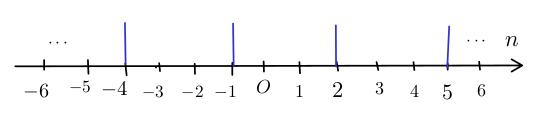
\includegraphics[width=0.46\textwidth]{d.jpg}
			\caption{Sketch $x[n]$}\label{fig:re11}

		\end{figure}
Dễ thấy $N_{0}=3$, vậy $\Omega_{0}=\frac{2\pi}{3}$, ta chọn đoạn $<N_{0}>=[0,2]$ (các bạn có thể chọn các đoạn khác) và thay trực tiếp công thức tính $c_{k}$ ở trên:
\begin{equation*}
\begin{split}
	c_{k}=\frac{1}{3}\sum_{n=0}^2 x[n]e^{-jk\Omega_{0}n}=\frac{1}{3}e^{-jk\frac{4\pi}{3}}
\end{split}
\end{equation*}
Tương tự như tín hiệu liên tục, ta cũng có thể vẽ phổ biên độ và pha của tín hiệu rời rạc \textbf{với lưu ý phổ tuần hoàn với chu kì cơ sở $N_{0}$}.
\\ Suy ngẫm: các bạn hãy tự vẽ phổ của tín hiệu $x[n]$ trên.
\end{frame}
\begin{frame}{Chuỗi Fourier (FS)}
\begin{itemize}
	\item[-] Tính chất chuỗi Fourier rời rạc
\end{itemize}
\begin{block}{Discrete-time Fourier Series Pair}
	\begin{equation*}
		\begin{split}
			x[n]&=\sum_{k=<N_{0}>}c_{k}e^{jk\Omega_{0}n}\\
			c_{k}&=\frac{1}{N_{0}}\sum_{n=<N_{0}>}x[n]e^{-jk\Omega_{0}n}
\end{split}
\end{equation*}
\end{block}
\subsubsection{Tính chất chuỗi Fourier rời rạc}
Tương tự như CTFS, DTFS cũng có các tính chất sau (chúng ta chỉ tổng quát hóa tính chất từ miền liên tục sang rời rạc và không chứng minh lại)
với $$\mathscr{FS}(x[n])=a_{k}\; , \mathscr{FS}(y[n])=b_{k}$$
\begin{enumerate}
	\item[1] Tính tuyến tính: $$\mathscr{FS}(\alpha x[n]+\beta y[n])=\alpha\mathscr{FS}(x[n])+\beta\mathscr{FS}(y[n])$$
	\item[2] Dịch thời gian: $$\mathscr{FS}(x[n-N_{0}])=a_{k}e^{-jk\Omega_{0}N_{0}}$$
\end{enumerate}
\end{frame}
\begin{frame}{Chuỗi Fourier (FS)}
\begin{enumerate}
	\item[3] Lật tín hiệu $$\mathscr{FS}(x[-n])=a_{-k}$$
	\item[4] Phép tích thường (điều chế): $$\mathscr{FS}(x[n]y[n])=a_{k}*b_{k}$$
	\item[5] Đẳng thức năng lượng Parseval: $$\frac{1}{N_{0}}\sum_{\alert{n=<N_{0}>}}|x[n]|^2=\sum_{\alert{k=<N_{0}>}}|a_{k}|^2$$
\end{enumerate}
\begin{itemize}
	\item[-] Đáp ứng của hệ thống LTI với tín hiệu tuần hoàn
\end{itemize}
\subsubsection{Đáp ứng của hệ thống LTI với tín hiệu tuần hoàn}
 Tương tự như tín hiệu và hệ thống LTI liên tục, ta cũng có:
$$H(jk\Omega_{0})=\sum_{n=-\infty}^{+\infty}h[n]e^{-jk\Omega_{0}n}$$
$$y[n]=\sum_{k=-\infty}^{+\infty}y_{k}[n]=\sum_{k=-\infty}^{+\infty}x_{k}[n]H(jk\omega_{0})$$
\end{frame}
\begin{frame}{Biến đổi Fourier (FT)}
\section{Biến đổi Fourier (FT)}
\subsection{Biến đổi Fourier liên tục (CTFT)}
\begin{itemize}
	\item Biến đổi Fourier liên tục (CTFT)
\end{itemize}
\subsubsection{Khái niệm biến đổi Fourier liên tục}
\begin{itemize}
	\item[-] Khái niệm biến đổi Fourier liên tục
\end{itemize}
Dirichlet đã tổng quát hóa kết quả của Fourier để phân tích phổ của tín hiệu \textbf{liên tục không tuần hoàn} như sau:
\begin{figure}[h]
			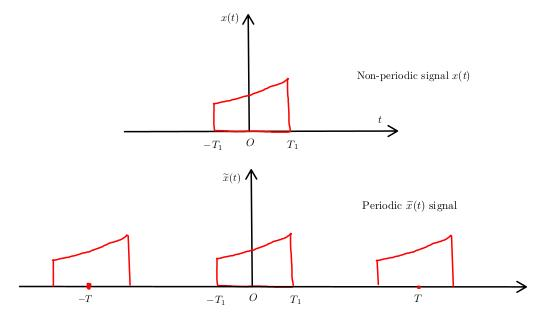
\includegraphics[width=0.46\textwidth]{signal.jpg}
			\caption{Form periodic signal $\widetilde{x}(t)$ from non-periodic signal $x(t)$}\label{fig:re11}

		\end{figure}
		\alert{Tín hiệu không tuần hoàn thì tuần hoàn với chu kì $T_{0}=+\infty$ !!!}
\\Áp dụng công thức chuỗi CTFS cho tín hiệu $\widetidle{x}(t)$, ta có:
\begin{equation*}
	\begin{split}
		\widetilde{x}(t)&=\sum_{k=-\infty}^{+\infty}a_{k}e^{jk\omega_{0}t}\\
		a_{k}&=\frac{1}{T_{0}}\int_{T_{0}}\widetilde{x}(t)e^{-jk\omega_{0}t}dt
	\end{split}
\end{equation*}
\end{frame}
\begin{frame}{Biến đổi Fourier (FT)}
	Khi $T_{0}\to+\infty$ thì hiển nhiên $\widetilde{x}(t)\to x(t)$, ta xét tích phân đoạn có độ dài $[\frac{-T_{0}}{2},\frac{T_{0}}{2}]$:
\begin{equation*}
a_{k}=\frac{1}{T_{0}}\int_{-\infty}^{+\infty}x(t)e^{-jk\omega_{0}t}dt
\end{equation*}
Ta định nghĩa:
$$X(j\omega)=\int_{-\infty}^{+\infty}x(t)e^{-j\omega t}dt$$
Quay ngược trở lại công thức tín hiệu gốc:
\begin{equation*}
\begin{split}
	\widetilde{x}(t)&=\sum_{k=-\infty}^{+\infty}a_{k}e^{jk\omega_{0}t}=\frac{1}{T_{0}}\sum_{k=-\infty}^{+\infty}X(jk\omega_{0})e^{jk\omega_{0}t}\\
			&=\sum_{k=-\infty}^{+\infty}\frac{1}{2\pi}X(jk\omega_{0})e^{jk\omega_{0}t}\omega_{0}
\end{split}
\end{equation*}
Hiển nhiên khi $T_{0}\to+\infty$ thì $\omega_{0}\to d\omega$, từ định nghĩa tổng Riemann, ta thu được:
$$x(t)=\frac{1}{2\pi}\int_{-\infty}^{+\infty}X(j\omega)e^{j\omega t}d\omega$$
Ví dụ: từ định nghĩa, hãy tìm biến đổi Fourier của tín hiệu sau với $a>0$:
$$x_{1}(t)=e^{-at}u(t)$$
$$x_{2}(t)=e^{at}u(t)$$

\end{frame}
\begin{frame}{Biến đổi Fourier (FT)}
\begin{equation*}
\begin{split}
	X_{1}(j\omega)&=\int_{-\infty}^{+\infty}x_{1}(t)e^{-j\omega t}dt=\int_{0}^{+\infty}e^{-at}e^{-j\omega t}dt=\frac{1}{a+j\omega}\\
	X_{2}(j\omega)&=\int_{-\infty}^{+\infty}x_{2}(t)e^{-j\omega t}dt=\int_{0}^{+\infty}e^{at}e^{-j\omega t}dt=\alert{+\infty}
\end{split}
\end{equation*}
Dễ thấy chỉ có tín hiệu $x_{1}(t)$ mới tồn tại biến đổi Fourier; còn tín hiệu $x_{2}(t)$ thì không do \textbf{tích phân phân kì, không hội tụ}.
\\ Dirichlet đã đưa ra 3 điều kiện để xác định sự tồn tại của biến đổi Fourier (các bạn có thể tra từ khóa Dirichlet's conditions); thế nhưng ta chỉ dùng điều kiện "lỏng" nhất, đó là \textbf{chỉ có tín hiệu năng lượng mới tồn tại biến đổi Fourier.} 
\begin{itemize}
	\item[-] Tính chất biến đổi Fourier liên tục:
\end{itemize}
\subsubsection{Tính chất biến đổi Fourier liên tục}
\begin{block}{Continuous-time Fourier Transform Pair}
If and only if $x(t)$ is an \textbf{\alert{energy signal:}}
\begin{equation*}
\begin{split}
	X(j\omega)&=\int_{-\infty}^{+\infty}x(t)e^{-j\omega t}dt\\
	x(t)&=\frac{1}{2\pi}\int_{-\infty}^{+\infty}X(j\omega)e^{j\omega t}d\omega
	\end{split}
\end{equation*}
\end{block}
 Trong quá trình giải bài tập thực chiến thì công thức $(2)$ không thường xuyên được sử dụng trong môn học này, mà thay vào đó ta tìm tín hiệu gốc $x(t)$ dựa vào tính chất của CTFT.
\end{frame}
\begin{frame}{Biến đổi Fourier (FT)}
Ta định nghĩa các phép toán CTFT của tín hiệu $x(t)$ như sau:
$$\mathscr{F}(x(t))=X(j\omega)$$
$$\mathscr{F}^{-1}(X(j\omega))=x(t)$$
Với tín hiệu $y(t)$ có:

$$\mathscr{F}(y(t))=Y(j\omega)$$
$$\mathscr{F}^{-1}(Y(j\omega))=y(t)$$
Ta lần lượt khảo sát các tính chất của CTFT gồm:
\begin{enumerate}
	\item[1] Tính tuyến tính:
\begin{equation*}
\begin{split}
	\mathscr{F}(\alpha x(t)+\beta y(t))&=\int_{-\infty}^{+\infty}[\alpha x(t)+\beta y(t)]e^{-j\omega t}dt\\
					   &=\alpha \int_{-\infty}^{+\infty}x(t)e^{-j\omega t}dt+\beta\int_{-\infty}^{+\infty}y(t)e^{-j\omega t}dt\\
					   &= \alpha\mathscr{F}(x(t))+\beta\mathscr{F}(y(t))\\
					   &= \alpha X(j\omega)+\beta Y(j\omega)
\end{split}
\end{equation*}
	\item[2] Dịch thời gian:
\begin{equation*}
\begin{split}
	\mathscr{F}(x(t-t_{0}))&=\int_{-\infty}^{+\infty}x(t-t_{0})e^{-j\omega t}dt=\int_{-\infty}^{+\infty}x(t-t_{0})e^{-j\omega (t-t_{0})}e^{-j\omega t_{0}}d(t-t_{0})\\
			       &=\mathscr{F}(x(t))e^{-j\omega t_{0}}=X(j\omega)e^{-j\omega t_{0}}
\end{split}
\end{equation*}
\end{enumerate}
\end{frame}
\begin{frame}{Biến đổi Fourier (FT)}
\begin{enumerate}
	\item[3] Dịch tần số:
\begin{equation*}
\begin{split}
	\mathscr{F}^{-1}(X(j(\omega-\omega_{0})))&=\frac{1}{2\pi}\int_{-\infty}^{+\infty}X(j(\omega-\omega_{0}))e^{j\omega t}d\omega \\&=\frac{1}{2\pi}\int_{-\infty}^{+\infty}X(j(\omega-\omega_{0}))e^{j(\omega-\omega_{0})t}e^{j\omega_{0}t}d(\omega-\omega_{0})\\&=x(t)e^{j\omega_{0}t}
\end{split}
\end{equation*}
$$\Leftrightarrow \mathscr{F}(x(t)e^{j\omega_{0}t})=X(j(\omega-\omega_{0}))$$
\item[4] Phép đạo hàm trong miền thời gian:
\begin{equation*}
\begin{split}
	\mathscr{F}\left(\frac{dx(t)}{dt}\right)&=\int_{-\infty}^{+\infty}\left(\frac{dx(t)}{dt}\right)e^{-j\omega t}dt=\int_{-\infty}^{+\infty}\left[\frac{j\omega}{2\pi}\int_{-\infty}^{+\infty}X(j\omega)e^{j\omega t}d\omega\right]e^{-j\omega t}dt\\&= j\omega\int_{-\infty}^{+\infty}x(t)e^{-j\omega t}dt=j\omega X(j\omega)
\end{split}
\end{equation*}
\item[5] Phép tích phân trong miền thời gian:
\begin{equation*}
\begin{split}
	\mathscr{F}\left(\int_{-\infty}^{t}x(\tau)d\tau\right)&=\int_{-\infty}^{+\infty}\left[\int_{-\infty}^{t}x(\tau)d\tau\right]e^{-j\omega t}dt\\
							      &=\int_{-\infty}^{+\infty}\left[\frac{1}{2\pi j\omega}\int_{-\infty}^{+\infty}X(j\omega)e^{j\omega t}d\omega\right]e^{-j\omega t}dt=\frac{X(j\omega)}{j\omega}
\end{split}
\end{equation*}
\end{enumerate}
\end{frame}
\begin{frame}{Biến đổi Fourier (FT)}
\begin{enumerate}
\item[6] Phép tích thường (điều chế):
\begin{equation*}
\begin{split}
	\mathscr{F}(x(t)y(t))&=\int_{-\infty}^{+\infty}[x(t)y(t)]e^{-j\omega t}dt=\int_{-\infty}^{+\infty}\frac{1}{2\pi}\left[\int_{-\infty}^{+\infty}X(jp)e^{jpt}dp\right]y(t)e^{-j\omega t}dt\\
			     &=\alert{\int_{-\infty}^{+\infty}\frac{1}{2\pi}X(jp)\left[\int_{-\infty}^{+\infty}y(t)e^{j(p-\omega)t} dt\right]dp}\\
			     &=\int_{-\infty}^{+\infty}\frac{1}{2\pi}X(jp)\left[\int_{-\infty}^{+\infty}y(t)e^{-j(\omega-p)t} dt\right]dp\\
			     &=\int_{-\infty}^{+\infty}\frac{1}{2\pi}X(jp)Y(j(\omega-p))dp\\
			     &=\frac{1}{2\pi}X(j\omega)*Y(j\omega)
\end{split}
\end{equation*}
\item[7] Phép đạo hàm trong miền tần số:
	\begin{equation*}
	\begin{split}
		\mathscr{F}^{-1}\left(\frac{dX(j\omega)}{d\omega}\right)=\mathscr{F}^{-1}\left(-jt\int_{-\infty}^{+\infty}x(t)e^{-j\omega t}dt\right)=\mathscr{F}^{-1}(-jtX(j\omega))=-jtx(t)
	\end{split}
\end{equation*}
\item[8] Phép đối ngẫu: 
\begin{equation*}
\begin{split}
\mathscr{F}(X(t))=2\pi x(-\omega)
\end{split}
\end{equation*}
\end{enumerate}
\end{frame}
\begin{frame}{Biến đổi Fourier (FT)}
\begin{enumerate}
	\item[] Phép đối ngẫu tương đối tricky và ý tưởng chứng minh không tự nhiên:
		\begin{equation*}
\begin{split}
	x(t)=\frac{1}{2\pi}\int_{-\infty}^{+\infty}X(j\omega)e^{j\omega t}d\omega\Leftrightarrow 2\pi x(t)=\int_{-\infty}^{+\infty}X(j\omega)e^{j\omega t}d\omega
\end{split}
		\end{equation*}
Đổi $t$ thành $-t$ và hoán đổi $t$ và $\omega$, ta lần lượt thu được:
\begin{equation*}
\begin{split}
	2\pi x(-t)&=\int_{-\infty}^{+\infty}X(j\omega)e^{-j\omega t}d\omega\\
	\Leftrightarrow 2\pi x(-\omega)&=\int_{-\infty}^{+\infty}X(t)e^{-j\omega t}dt=\mathscr{F}(X(t))
\end{split}
\end{equation*}
\item[9] Phép tích chập trong miền thời gian:
\begin{equation*}
\begin{split}
	\mathscr{F}(x(t)*y(t))&=\int_{-\infty}^{+\infty}[x(t)*y(t)]e^{-j\omega t}dt=\int_{-\infty}^{+\infty}\left[\int_{-\infty}^{+\infty}x(\tau)y(t-\tau)d\tau\right]e^{-j\omega t}dt\\
			      &=\alert{\int_{-\infty}^{+\infty}x(\tau)\left[\int_{-\infty}^{+\infty}y(t-\tau)e^{-j\omega (t-\tau)} d(t-\tau)\right]e^{-j\omega \tau}d\tau}\\
			      &=\int_{-\infty}^{+\infty}x(\tau)Y(j\omega)e^{-j\omega \tau}d\tau \\
			      &=X(j\omega)Y(j\omega)
\end{split}
\end{equation*}
\end{enumerate}
\end{frame}
\begin{frame}{Biến đổi Fourier (FT)}
\begin{enumerate}
	\item[10] Co giãn trong miền thời gian, với $a>0$ ($a<0$ chứng minh tương tự):
\begin{equation*}
\begin{split}
	\mathscr{F}(x(at))&=\int_{-\infty}^{+\infty}x(at)e^{-j\omega t}dt=\frac{1}{a}\int_{-\infty}^{+\infty}x(at)e^{-j\omega t}d(at)\\
			  &=\frac{1}{a}\int_{-\infty}^{+\infty}x(t)e^{\frac{-j\omega t}{a}}dt=\frac{1}{a}X\left(\frac{\omega}{a}\right)
\end{split}
\end{equation*}
Trường hợp $a<0$ các bạn chỉ cần đảo cận tích phân ngược lại là xong, tổng quát ta có với trường hợp $a$ bất kì:
$$\mathscr{F}\left(x(at)\right)=\frac{1}{|a|}X\left(\frac{\omega}{a}\right)$$
\item[11] Đẳng thức năng lượng Parseval:
	$$\int_{-\infty}^{+\infty}|x(t)|^2 dt=\frac{1}{2\pi}\int_{-\infty}^{+\infty}|X(j\omega)|^2d\omega$$
	Đẳng thức này rất khó chứng minh nên ta chỉ cần liên hệ nó với công thức tương tự trong phần CTFS và nhớ mà thôi.
\end{enumerate}
Suy ngẫm: ngoại trừ tính chất 11, các bạn hãy tự chứng minh lại \alert{toàn bộ} phép toán trên để khắc sâu bản chất của phép biến đổi Fourier về mặt toán học.
\end{frame}
\begin{frame}{Biến đổi Fourier (FT)}
Ví dụ: sử dụng phép đối ngẫu:
\begin{equation*}
\begin{split}
	\mathscr{F}(\delta(t))&=\int_{-\infty}^{+\infty}\delta(t)e^{-j\omega t}dt=1 \\
	\Rightarrow \mathscr{F}(1)&=2\pi\delta(-\omega)=2\pi\delta(\omega)
\end{split}
\end{equation*}
Tiếp tục sử dụng phép dịch tần số $\omega_{0}$:
\begin{equation*}
	\begin{split}
		\mathscr{F}(1)&=2\pi\delta(\omega)\Rightarrow \mathscr{F}^{-1}(2\pi\delta(\omega-\omega_{0}))=e^{j\omega_{0}t}\\
		\Rightarrow & \mathscr{F}(e^{j\omega_{0}t})=2\pi\delta(\omega-\omega_{0})
	\end{split}
\end{equation*}
Về mặt \alert{biểu thức toán học} sử dụng tính chất tuyến tính ta thu được:
$$\mathscr{F}(\cos{(\omega_{0}t)})=\mathscr{F}\left[\frac{1}{2}\left(e^{j\omega_{0}t}+e^{-j\omega_{0}t}\right)\right]=\pi(\delta(\omega-\omega_{0})+\delta(\omega+\omega_{0}))$$
Suy ngẫm: các bạn hãy tìm CTFT của tín hiệu sau theo gợi ý với $a>0$:
$$x(t)=e^{-at}\cos{(\omega_{0}t)}u(t)$$
Gợi ý: dùng công thức Euler để tách $\cos(\omega_{0}t)$ ra thành tổng hai thành phần mũ phức, đến đây ta có hai hướng làm: tìm CTFT của tín hiệu $e^{-at}u(t)$ rồi sau đó dùng tính chất dịch tần số; hoặc tìm CTFT của tín hiệu phức $e^{\pm j\omega_{0}t}$ rồi sau đó dùng tính chất dịch tần số.
\end{frame}
\begin{frame}{Biến đổi Fourier (FT)}
\begin{figure}[h]
			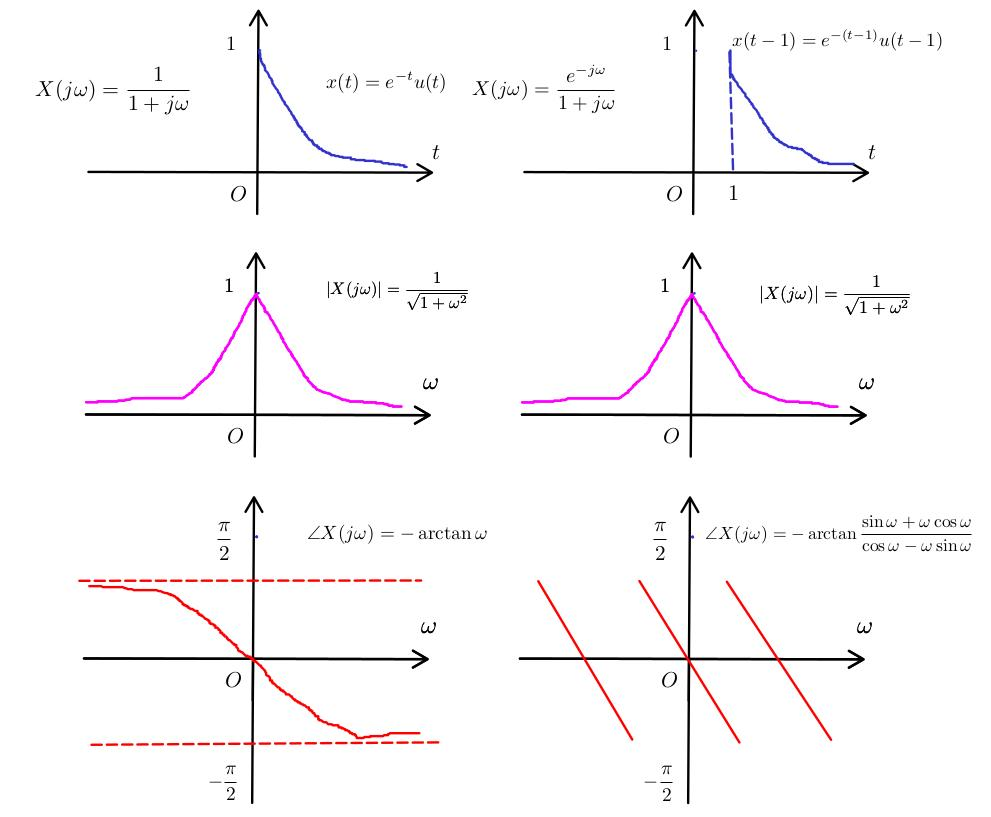
\includegraphics[width=0.8\textwidth]{spectrum.jpg}
			\caption{Time-shifting property visualization}\label{fig:re11}

		\end{figure}

\end{frame}
\begin{frame}{Biến đổi Fourier (FT)}
\begin{figure}[h]
			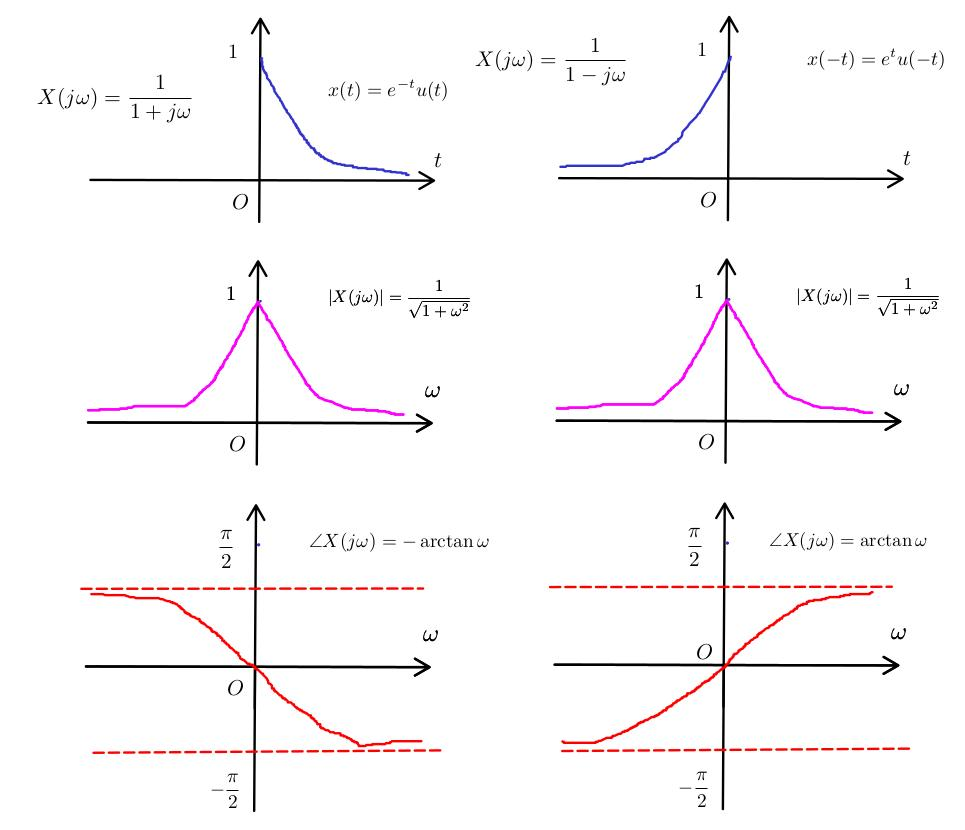
\includegraphics[width=0.8\textwidth]{spec.jpg}
			\caption{Time-scaling (flipping) property visualization}\label{fig:re11}

		\end{figure}

\end{frame}
\begin{frame}{Biến đổi Fourier (FT)}
Suy ngẫm: hãy tìm biến đổi Fourier của tín hiệu $x(t)=e^{-|a|t}$ với $a>0$, vẽ tay phổ biên độ và phổ pha của nó. Quan sát dạng biểu thức của tín hiệu gốc, hãy thử các tính chất như lật, giãn,... trong 10 tính chất đã cho để xem dạng phổ tín hiệu thay đổi như thế nào (các bạn nên tự vẽ tay trước sau đó dùng Matlab hoặc GNU Octave kiểm tra lại kết quả sau).
\\ Như đã đề cập ở phần trước, phần lớn các bài tập liên quan đến tìm tín hiệu gốc $x(t)$ của phép biến đổi Fourier ngược đa phần dùng tính chất của CTFT chứ không dùng công thức. Đây là dạng bài tập khó và cần phải luyện tập tương đối nhiều để thuần thục.
\\ Ví dụ:
\begin{equation*}
\begin{split}
	\mathscr{F}^{-1}\left(\frac{j\omega}{(1+j\omega)^2}\right)=?
\end{split}
\end{equation*}
Từ CTFT cơ bản:
$$\mathscr{F}(e^{-t}u(t))=\frac{1}{1+j\omega}$$
Sử dụng tính chất phép đạo hàm trong miền tần số, ta có:
$$\mathscr{F}(te^{-t}u(t))=\frac{1}{(1+j\omega)^2}$$
Sử dụng tính chất phép đạo hàm trong miền thời gian, ta có:
$$\mathscr{F}\left[{\frac{d(te^{-t}u(t))}{dt}}\right]=\frac{j\omega}{(1+j\omega)^2}$$
\end{frame}
\begin{frame}{Biến đổi Fourier (FT)}
Vậy ta thu được:

$$	\mathscr{F}^{-1}\left(\frac{j\omega}{(1+j\omega)^2}\right)=(1-t)e^{-t}u(t)$$
Suy ngẫm: hãy tự chứng minh lại bảng CTFT của các tín hiệu thường gặp sau (với $a>0$):
\begin{center}
\begin{tabular}{ |l|l| } 
 \hline
 $f(t)$ & $F(j\omega)$ \\ 
 $e^{-at}u(t)$ & $\frac{1}{a+j\omega}$  \\ 
 $e^{at}u(-t)$ &   $\frac{1}{a-j\omega}$ \\ 
 $e^{-|a|t}$ & $\frac{2a}{a^2+\omega^2}$\\
 $te^{-at}u(t)$ & $\frac{1}{(a+j\omega)^2}$\\
 $\delta(t)$ & $1$\\
 $1$ & $2\pi\delta(\omega)$ \\
 $e^{j\omega_{0}t}$ & $2\pi\delta(\omega-\omega_{0})$\\
 $\cos(\omega_{0}t)$ & $\pi(\delta(\omega+\omega_{0})+\delta(\omega-\omega_{0}))$\\
 $\sin(\omega_{0}t)$ & $j\pi(\delta(\omega+\omega_{0})-\delta(\omega-\omega_{0}))$\\
 $e^{-at}\sin(\omega_{0}t)u(t)$ & $\frac{\omega_{0}}{(a+j\omega)^2+\omega_{0}^2}$\\
 $e^{-at}\cos(\omega_{0}t)u(t)$ & $\frac{a+j\omega}{(a+j\omega)^2+\omega_{0}^2}$\\

 \hline
\end{tabular}
\end{center}
Mở rộng (optional): mặc dù không gặp trong môn học này (sẽ gặp rất nhiều trong môn Xử lý tín hiệu số) nhưng các bạn có thể thử tìm:
$$\mathscr{F}(rect(t))=\mathscr{F}\left(\prod(t)\right)=?$$
\end{frame}
\begin{frame}{Biến đổi Fourier (FT)}
	\begin{itemize}
		\item[-] Phân tích hệ thống LTI liên tục
	\end{itemize}
\subsubsection{Phân tích hệ thống LTI liên tục}
Ngoài ra, CTFT còn mở ra cho chúng ta một công cụ cực kì mạnh mẽ để phân tích
hệ thống LTI do \alert{phép tích chập trong miền thời gian tương ứng với phép nhân đại số
trong miền tần số}.
\\Ví dụ: xác định \alert{lối vào} của hệ thống có đáp ứng xung và đáp ứng lối ra được cho như sau:
$$h(t)=e^{-t}u(t)$$
$$y(t)=e^{-2t}u(t)$$
Bài toán này gần như \textbf{bất khả thi} nếu giải theo phương pháp tích chập đã học ở \alert{Chương 2}, ta chỉ còn cách giải theo đáp ứng tần số:
\\ Dễ thấy từ tính chất của hệ thống LTI:
$$x(t)*h(t)=y(t)\Rightarrow \mathscr{F}(x(t)*h(t))=\mathscr{F}(y(t))$$
$$\Rightarrow X(j\omega)H(j\omega)=Y(j\omega)\Rightarrow X(j\omega)=\frac{Y(j\omega)}{H(j\omega)}$$
Và ta có: $$x(t)=\mathscr{F}^{-1}(X(j\omega))=\mathscr{F}^{-1}\left[\frac{Y(j\omega)}{H(j\omega)}\right]=\mathscr{F}^{-1}\left(\frac{1+j\omega}{2+j\omega}\right)=\mathscr{F}^{-1}\left(1-\frac{1}{2+j\omega}\right)$$
Sử dụng bảng CTFT đã cho ở trên (các bạn phải \textbf{cực kì thông thạo bảng CTFT}), ta dễ dàng xác định được: $x(t)=1-e^{-2t}u(t)$
\end{frame}
\begin{frame}{Biến đổi Fourier (FT)}
\subsection{Biến đổi Fourier rời rạc (DTFT)}
\begin{itemize}
	\item Biến đổi Fourier rời rạc (DTFT)
\end{itemize}
\subsubsection{Khái niệm biến đổi Fourier rời rạc}
\begin{itemize}
	\item[-] Khái niệm biến đổi Fourier rời rạc
\end{itemize}
Do ý tưởng của biến đổi Fourier rời rạc (DTFT) hoàn toàn tương tự với CTFT, nên ở đây ta chỉ đưa ra cặp công thức và ví dụ cơ bản:
\begin{equation*}
\begin{split}
X(j\Omega)&=\sum_{n=-\infty}^{+\infty}x[n]e^{-j\omega n}\\
x[n]&=\frac{1}{2\pi}\int_{2\pi}X(j\Omega)e^{jn\omega}d\omega
\end{split}
\end{equation*}
Tương tự như CTFT ta cũng thử tìm DTFT của hai tín hiệu rời rạc sau:
$$x_{1}[n]=2^{n}u[n]$$
$$x_{2}[n]=2^{-n}u[n]$$
Dễ thấy:
\begin{equation*}
\begin{split}
	X_{1}(j\Omega)&=\sum_{n=-\infty}^{+\infty}x_{1}[n]e^{-j\omega n}=\sum_{n=0}^{+\infty}2^n e^{-j\omega n}=\alert{+\infty}\\
	X_{2}(j\Omega)&=\sum_{n=-\infty}^{+\infty}x_{2}[n]e^{-j\omega n}=\sum_{n=0}^{+\infty}2^{-n} e^{-j\omega n}=
	\frac{1}{1-\frac{1}{2}e^{-j\omega}}
\end{split}
\end{equation*}
\end{frame}
\begin{frame}{Biến đổi Fourier (FT)}
Vậy điều kiện Dirichlet cũng nghiệm đúng với DTFT, chỉ có tín hiệu năng lượng mới tồn tại DTFT.
\subsubsection{Tính chất biến đổi Fourier rời rạc}
\begin{itemize}
	\item[-] Tính chất biến đổi Fourier rời rạc
\end{itemize}
\begin{block}{Discrete-time Fourier Transform}
If and only if $x[n]$ is \alert{an energy signal}:
\begin{equation*}
	\begin{split}
X(j\Omega)&=\sum_{n=-\infty}^{+\infty}x[n]e^{-j\omega n}\\
x[n]&=\frac{1}{2\pi}\int_{2\pi}X(j\Omega)e^{jn\omega}d\omega
\end{split}
\end{equation*}
\end{block}
Tương tự như CTFT, đa phần khi giải bài tập thực chiến ta không thường xuyên dùng công thức (2) mà thay vào đó tìm tín hiệu gốc $x[n]$ dựa trên các tính chất của DTFT.
\\ Ở đây, thay vì chứng minh lại toàn bộ tính chất DTFT, ta sẽ chỉ dẫn ra các công thức cơ bản nhất có dạng giống và tương tự với CTFT cho dễ nhớ. Các bạn không cần nhớ hết mà chỉ cần nhớ được các tính chất kí hiệu màu đỏ (sẽ gặp lại rất thường xuyên trong \alert{Chương 5} và môn Xử lý tín hiệu số), còn lại thì chỉ cần tham khảo mà thôi.
\end{frame}
\begin{frame}{Biến đổi Fourier (FT)}
\begin{enumerate}
	\item[1] \alert{Dịch trong miền thời gian:}
\alert{$$\mathscr{F}(x[n-n_{0}])=X(j\Omega)e^{-j\omega n_{0}}$$}
\item[2] \alert{Dịch trong miền tần số: }
	\alert{$$\mathscr{F}(x[n]e^{j\Omega n_{0}})=X(j(\Omega-\Omega_{0}))$$}
\item[3] \alert{Lật tín hiệu:}
	\alert{$$\mathscr{F}(x[-n])=X(-j\Omega)$$}
\item[4] Sai phân trong miền thời gian:
	$$\mathscr{F}(x[n+1]-x[n])=j\Omega X(j\Omega)$$
\item[5] \alert{Đạo hàm trong miền tần số:}
	\alert{$$\mathscr{F}(-jnx[n])=\frac{dX(j\Omega)}{d\Omega}$$}
\item[6] Tích thường (tích điều chế):
	$$\mathscr{F}(x[n]y[n])=\frac{1}{2\pi}X(j\Omega)\circledast Y(j\Omega)$$
\end{enumerate}
\end{frame}
\begin{frame}{Biến đổi Fourier (FT)}
\begin{enumerate}
	\item[7] \alert{Tích chập trong miền thời gian:}
		\alert{$$\mathscr{F}(x[n]*y[n])=X(j\Omega)Y(j\Omega)$$}
\end{enumerate}
Ví dụ: tìm DTFT của tín hiệu
$$x[n]=3^{-n}u[n+2]$$
Ta có: 
$$\mathscr{F}(3^{-n}u[n])=\frac{1}{1-\frac{1}{3}e^{-j\Omega }}$$
Sử dụng tính chất dịch trong miền thời gian:
$$\mathscr{F}(3^{-(n+2)}u[n+2])=\frac{e^{j2\Omega}}{1-\frac{1}{3}e^{-j\Omega }}$$
Vậy ta suy ra:
$$\mathscr{F}(3^{-n}u[n+2])=\frac{9e^{j2\Omega}}{1-\frac{1}{3}e^{-j\Omega }}$$
\end{frame}
\begin{frame}{Biến đổi Fourier (FT)}
Ta có bảng DTFT cơ bản sau (rất ngắn so với CTFT, do DTFT không thường xuyên được hỏi nhiều trong đề thi trường mình) ($|a|<1$):
\begin{center}
\begin{tabular}{ |l|l| } 
 \hline
 $x[n]$ & $X(j\Omega)$\\ 
 $a^{n}u[n]$ & $\frac{1}{1-ae^{-j\Omega }}$ \\ 
 $\delta[n]$ & $1$ \\ 
 $\delta[n-n_{0}]$ & $e^{-j\Omega n_{0}}$\\
 \hline
\end{tabular}
\end{center}
Suy ngẫm: hãy tìm DTFT của tín hiệu sau với ($|a|<1$)
$$\mathscr{F}((n+1)a^n u[n])=?$$
\begin{itemize}
	\item[-] Phân tích hệ thống LTI rời rạc
\end{itemize}
\subsubsection{Phân tích hệ thống LTI rời rạc}
Tương tự như hệ thống LTI liên tục, ta có thể dùng phương pháp đáp ứng tần số để phân tích hệ thống rời rạc.
\\ Ví dụ: xác định tín hiệu lối vào của hệ thống LTI rời rạc có đáp ứng xung và đáp ứng lối ra lần lượt: $$h[n]=2^{-n}u[n]$$ $$y[n]=3^{-n}u[n]$$
Ta có: 
\begin{equation*}
\begin{split}
	x[n]&=\mathscr{F}^{-1}(X(j\Omega))=\mathscr{F}^{-1}\left(\frac{Y(j\Omega)}{H(j\Omega)}\right)=\mathscr{F}^{-1}\left(\frac{1-2^{-1}e^{-j\Omega}}{1-3^{-1}e^{-j\Omega}}\right)\\
	    &=\mathscr{F}^{-1}\left(1-\frac{1}{6}\frac{1}{1-3^{-1}e^{-j\Omega}}\right)=\delta[n]-\frac{1}{6}3^{-n}u[n]
\end{split}
\end{equation*}
\end{frame}
\end{document}
